\section{Locked Three-Dimensional Validation}
\subsection{Common physical problem and comparison}
The experiments use the same vector-Maxwell DDA state and derivative operators throughout; general DDA background is given in~\cite{r11}. Six transverse plane-wave illuminations and 64 dual-polarization receivers sample the scattered field. The inverse grid has $12^3$ cells in a box of side 1.5, with $k_0=2$; truth data use a $14^3$ grid. Both grids use the same DDA family. The material coordinates are volume-orthonormal Gaussian or voxel tangents, with the true polarizability derivative retained. The full forward residual and injection are common to both policies; only the tangent-current space changes. Current ranks $k=4,8,16$ are actual shared complex columns, distinct from the real material dimension. The Supplement provides the implemented dyadic, acquisition, gauges, and hash-locked protocol.

We compare the unchanged receiver backbone with the frozen verified-exchange rule. Each object contributes the initial linearization, saved iteration index 3, and last saved linearization. A complete object therefore has nine state--rank cells. We aggregate absolute full-GN gaps within an object before dividing by its receiver total. The independent aggregation unit is the object, not a state or rank. A 10,000-draw object bootstrap uses the predeclared seed 20261002.

\subsection{Original objects and additional-object validation}
The original smooth Gaussian, near-contact Gaussian, layered voxel, and asymmetric voxel objects give 35 improved cells and one equal cell out of 36. Their object-summed gap ratios are 0.1904,0.6538,0.2776, and 0.4181; the median 0.3478 represents a 65.2\% reduction. The physical threshold replay preserves all these results.

Before additional results, we locked the rule, thresholds, seeds, and all eleven remaining compatible objects. Ten objects provide complete nine-cell coverage and all ten improve. Their median object-summed ratio is 0.4928, a 50.7\% reduction; the interquartile range is [0.3314,0.5588] and the object-bootstrap 95\% interval for the median is [0.3133,0.5647]. The remaining asymmetric voxel object completes six early/middle cells, with ratio 0.4925. Its late receiver endpoint fails the frozen normal-residual check at the first budget; the two subsequent budgets are not run. All three unavailable cells remain in the 99-cell denominator.

Among the 96 audited additional-object cells, 95 improve, one is equal within the evaluation floor, and none worsen. Absolute receiver gaps span $2.74\times10^{-7}$--$3.09\times10^{-3}$; exchange gaps span $8.73\times10^{-8}$--$8.36\times10^{-4}$. The smallest receiver denominator exceeds its evaluation floor by $6.31\times10^9$, and the maximum full-reference true normal residual is $9.55\times10^{-12}$. The improvement is resolved in the stored absolute quantities, rather than created by dividing two floor-level risks. Figure~\ref{fig:locked-primary} reports both ratios and absolute gaps.

\begin{figure*}[t]\centering
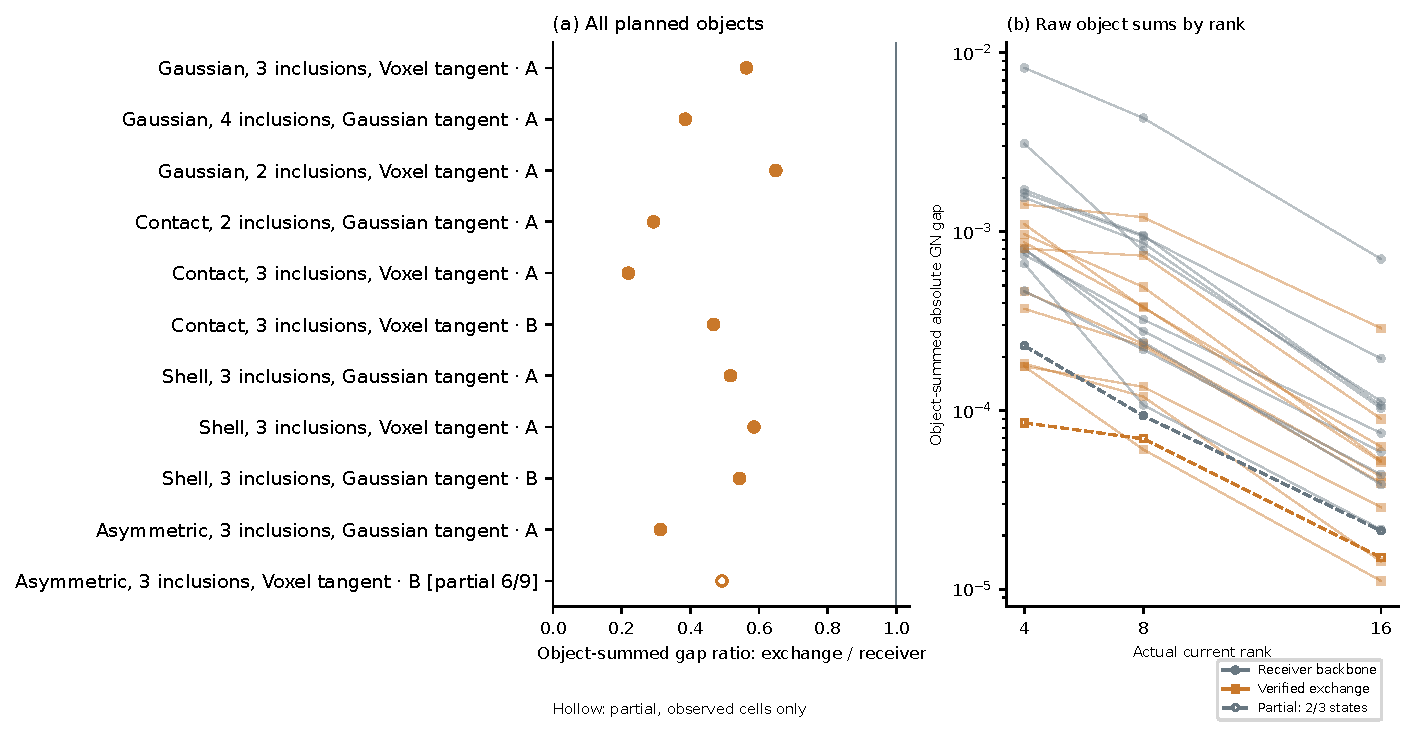
\includegraphics[width=.92\textwidth]{figures/closure_validation_v2/Figure1_primary_overview.pdf}
\caption{Frozen-rule validation on all planned additional objects. Left: object-summed full-GN gap ratios; filled markers are ten complete objects, while the hollow marker uses six of nine cells from the remaining object. Right: paired absolute gap sums by current rank; dashed curves retain that object's two available states. Geometry labels distinguish smooth profiles, contact structures, shells, and asymmetric structures; the complete representation mapping is in the Supplement. These quantities measure frozen material-step fidelity.}\label{fig:locked-primary}
\end{figure*}

These additional objects were historically studied in a broader current-ranking investigation. Inspected records show no object-specific use in historical exchange-teacher or pilot-network development, but complete blind independence cannot be established from their historical exposure. We therefore describe this test as locked-rule validation on additional previously studied Maxwell objects. The bootstrap summarizes this fixed object set; it is not a distribution-free generalization guarantee.

\subsection{Noisy residuals}
Four objects were preselected by geometry and representation: smooth voxel, near-contact Gaussian, shell Gaussian, and asymmetric voxel. Their middle-state physics is fixed while 1\% and 3\% relative complex noise changes the residual, with three independent realizations at each level. Every noisy residual receives its own offline full-GN reference after online selection. All 72 planned cells are audited: 71 improve and one abstains with an unchanged gap. The median object-summed ratios are 0.3307 at 1\% and 0.4026 at 3\% (Table~\ref{tab:noise}).

The controller verifies 408 finalists and rejects 98 below the numerical threshold; 172 exchanges are accepted. Verification costs 2448 current right-hand sides for $Jd$, including rejected finalists. Selected directions change with the residual, so this evidence concerns retained update utility rather than invariance of selected modes. The limited four-object, middle-state test supports the effect at these two noise levels.

\begin{table}[t]\centering\caption{Noise: ratio of object-summed full-GN gaps. Each entry sums three realizations and three current ranks.}\label{tab:noise}
\begin{tabular}{lrr}\toprule
Geometry / material tangent&1\%&3\%\\\midrule
Smooth / voxel&0.3255&0.4384\\
Near-contact / Gaussian&0.0996&0.1873\\
Shell / Gaussian&0.3358&0.3667\\
Asymmetric / voxel&0.3687&0.5330\\\midrule
Object median&0.3307&0.4026\\\bottomrule
\end{tabular}
\end{table}

\subsection{Ranking, candidate coverage, and exchange paths}
An offline diagnostic enumerates every feasible initial one-out/one-in replacement in the fixed 154-atom dictionary, then follows at most three full-score greedy exchanges. Its labels are acquired after the online decisions and never change them. The 96 available cells are complete; the three cells excluded by the earlier endpoint failure remain unrun.

Across the ten complete additional objects, the reduced anchor's full-dictionary top choice captures 97.30--99.99\% of the summed positive initial-exchange opportunity (median 99.54\%). Restricting acquisition to the frozen 12-atom incoming pool captures 49.12--95.31\% (median 72.95\%). Thus candidate acquisition, rather than reduced ranking alone, is the larger limitation in this test. These are positive-gain-weighted initial-neighborhood captures, not the improvement fraction of the deployed multistep method. The separate bounded greedy path reaches a smaller final gap in 90 of 96 cells, the online path is smaller in five, and one agrees within the evaluation floor. A greedy path is a local diagnostic, not a global optimum; its difference from deployment combines coverage, ranking, and path interactions.


\subsection{Constrained nonlinear transfer}
Four objects were fixed by geometry and material representation before validation. At $k=8$, both policies use the same initialization, prior, damping schedule, material constraints and full-objective Armijo line search. Only the tangent-current policy changes. Three paired trajectories complete all 18 updates. Table~\ref{tab:nonlinear} reports their complete-volume material errors and held-out data errors.

\begin{table*}[t]\centering
\caption{Constrained nonlinear transfer: receiver $\rightarrow$ verified exchange. Material errors are relative full-volume norms. Child wall includes each policy's own physical setup, acquisition, all outer work and terminal evaluation. Each trajectory is timed once.}\label{tab:nonlinear}
\begin{tabular}{lrrrr}\toprule
Geometry / material tangent&Complex material&Real material&Imaginary material&Held-out data\\\midrule
Smooth / voxel&$0.3027\to0.2699$&$0.2811\to0.2516$&$0.7439\to0.6506$&$0.006637\to0.002836$\\
Near-contact / Gaussian&$0.6722\to0.6707$&$0.6810\to0.6835$&$0.4439\to0.2859$&$0.010521\to0.007080$\\
Shell / Gaussian&$0.6096\to0.5660$&$0.6081\to0.5651$&$0.6976\to0.6219$&$0.014190\to0.012179$\\\midrule
Geometry / material tangent&\multicolumn{2}{c}{Child wall (s)}&Wall ratio&Total full tangent RHS\\
Smooth / voxel&\multicolumn{2}{c}{$216.5\to579.9$}&2.68&$0\to708$\\
Near-contact / Gaussian&\multicolumn{2}{c}{$407.7\to710.5$}&1.74&$0\to744$\\
Shell / Gaussian&\multicolumn{2}{c}{$405.9\to592.3$}&1.46&$0\to744$\\\bottomrule
\end{tabular}
\end{table*}

Complex-material error decreases by 10.8\%, 0.22\%, and 7.16\%, respectively, and held-out errors decrease in all three pairs. The near-contact real-part error increases slightly, so improved data fit does not imply uniform component recovery. The fourth object's exchange trajectory retains 17 completed updates. Before update 18, its receiver-derived starting endpoint fails the fixed normal-residual check, stopping that exchange trajectory. The separate receiver-only baseline job is not run after the queue stops. The four-object denominator and both unavailable final endpoints remain explicit.

These trajectories support a limited reconstruction consequence of the frozen rule. They also separate fidelity from efficiency: the complete child-wall ratios range from 1.46 to 2.68. Extra tangent actions purchase checked material changes; faster imaging is not established.

\begin{figure*}[t]\centering
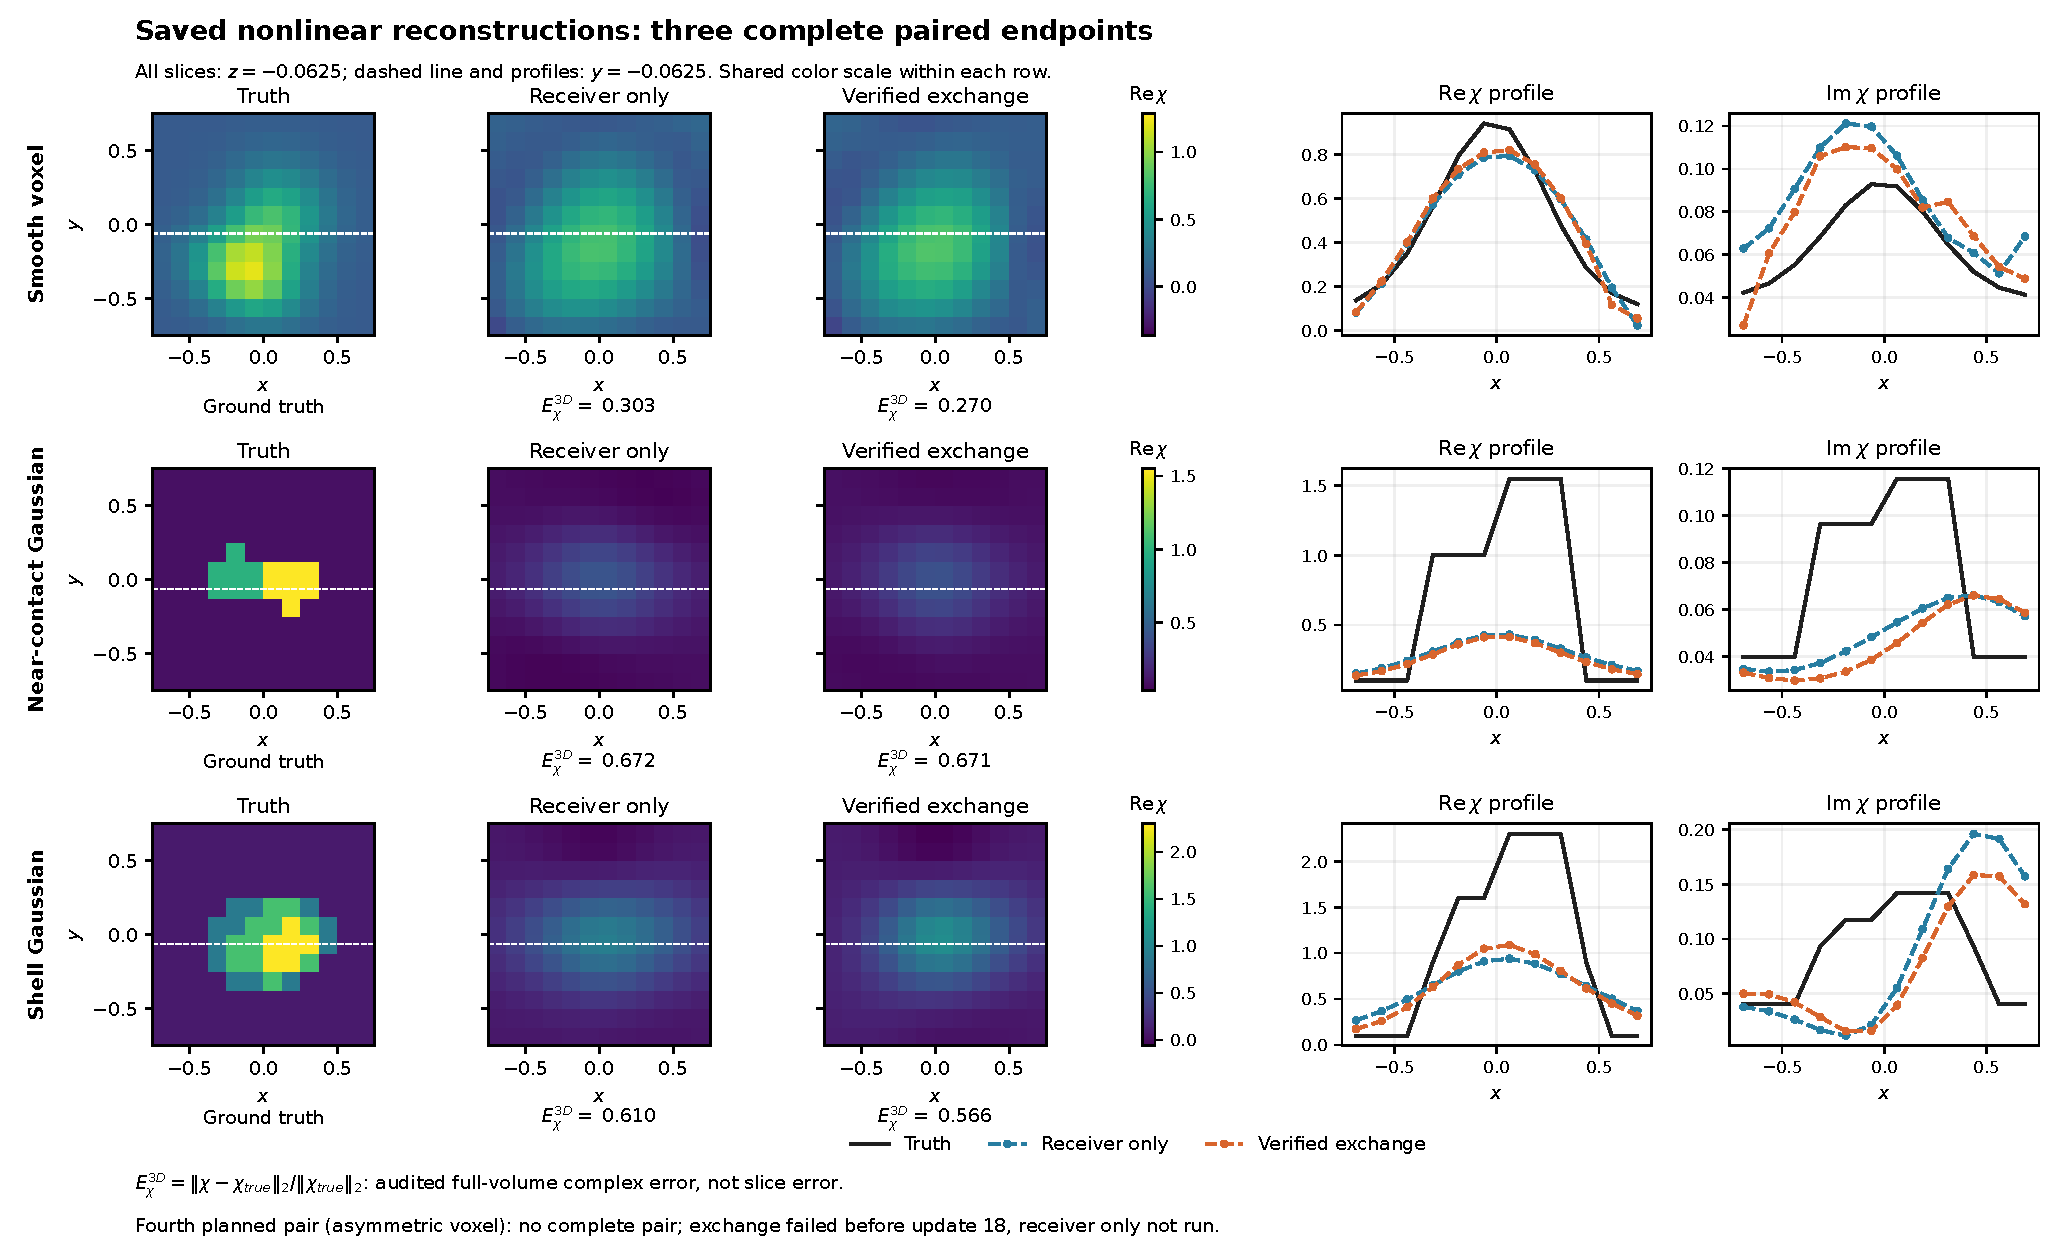
\includegraphics[width=.92\textwidth]{figures/nonlinear_closure_v1/nonlinear_reconstructions.pdf}
\caption{Complete nonlinear pairs at current rank eight. The real-material slices use the same central inverse-grid plane and a common color scale within each row; line profiles compare both real and imaginary contrast. These images accompany complete-volume errors in Table~\ref{tab:nonlinear}. The contact and shell peaks remain blurred despite improved data fit. The asymmetric voxel pair has no completed paired endpoint and is retained separately in the failure record.}\label{fig:nonlinear-slices}
\end{figure*}


\subsection{The added price of a current-space decision}
Exchange pays for the richer anchor, candidate acquisition, endpoint proposals and full directional checks beyond the unchanged receiver endpoint. The frozen workflow shares projected operators; a separate cold receiver-only build was not timed, so its warm selection wall is not an end-to-end baseline. The independently initialized nonlinear trajectories provide the all-in comparison: exchange takes 2.68, 1.74 and 1.46 times receiver-only child wall in the three complete pairs. The design purchases material-step fidelity with additional physics work.

Full campaign accounting, including historical carry, failed launches, verification, references and offline full-dictionary diagnostics, closes at 19,962.060~s (5.545~h). This is an execution-accounting total, rather than a per-solve runtime. The Supplement distinguishes additive occupation from nested stage and action counts; no acceleration follows from either a warm selection time or one reduced class of right-hand sides.


